\documentclass[12pt,]{article}


%\usepackage{baskervillef}%polskie znaki może nie

%flow chatry
\usepackage{tikz}
\usetikzlibrary{shapes.geometric, arrows}
\usepackage{amssymb}
\usepackage{float}

\title{Sprawozadanie lernicng}
\author{Tymon Łazowy}
\date{123,2123,12}


\tikzstyle{startstop} = [ellipse, rounded corners, minimum width=2cm, minimum height=1cm,text centered, draw=black,thick,fill=red!0]

\tikzstyle{io} = [trapezium,
trapezium stretches=true,
trapezium left angle=70,
trapezium right angle=110,
thick,minimum width=2cm,
minimum height=0.85cm,
text centered,
draw=black,
fill=blue!0]

\tikzstyle{process} = [rectangle,
minimum width=3cm,
minimum height=0.85cm,
text centered,
text width=3cm,draw=black,thick,fill=orange!0]

\tikzstyle{decision} = [diamond,minimum width=1cm, minimum height=1cm, text centered, draw=black, fill=green!0,thick,yshift=1.0]

\tikzstyle{arrow} = [thick,->,>=stealth]

\begin{document}
 D: a,b,c parametry $\in$ $\mathbb{R}$
 
 S: P, pole $\in$ $\mathbb{R}$
\begin{figure}[h]
   
    \caption{1.9 flowchart} 
    \centering  
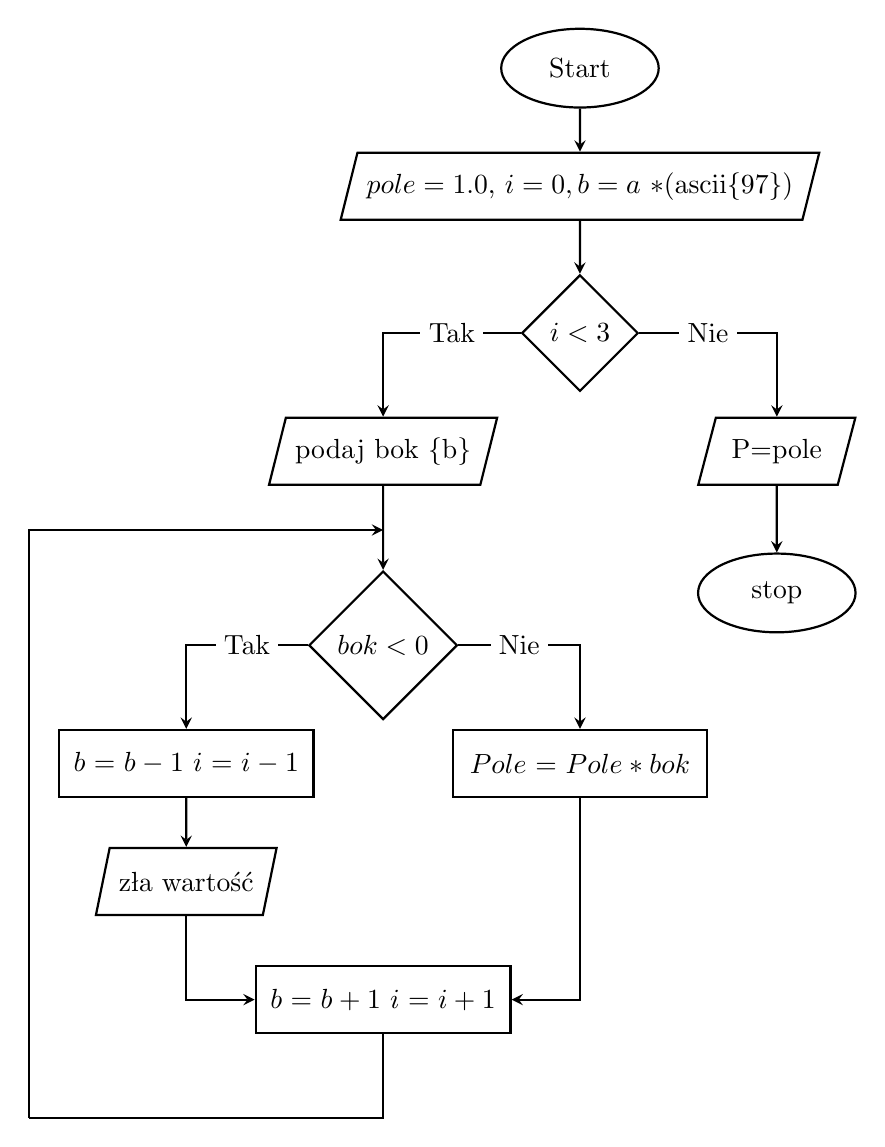
\begin{tikzpicture}[node distance=1.5cm]

\node (start) [startstop] {Start};
\node (in1) [io, below of=start,] {$pole=1.0$,  $i=0,b=a$  $\ast$(ascii\{97\})};
\node (dec1) [decision, below of=in1,yshift=-.4cm] {$i<3$};
\node (in2) [io, left of=dec1,yshift=-1.5cm,xshift=-1.cm] {podaj bok \{b\}};
\node (meet2)[coordinate,below of =in2,yshift=0.5cm]{};
\node (dec2) [decision, below of=meet2,] {$bok<0$};
\node (tak1) [process, left of=dec2,yshift=-1.5cm,xshift=-1.cm] {$b=b-1$ $i=i-1$};
\node (out1) [io, below of=tak1,] {zła wartość};
\node (nie1) [process, right of=dec2,yshift=-1.5cm,xshift=1.cm] {$Pole=Pole*bok$};
\node (pro2) [process, below of=dec2,yshift=-3cm] {$b=b+1$ $i=i+1$};
\node (out) [io, right of=dec1,yshift=-1.5cm,xshift=1.cm] {P=pole};
\node (stop) [startstop, below of=out,yshift=-0.3cm]{stop};
\node (meet)[coordinate,below of =pro2,xshift=-4.5cm]{};

\draw [arrow] (start) -- (in1);
\draw [arrow] (in1) -- (dec1);
\draw[arrow] (dec1) -| (out) node[pos=0.25,fill=white,inner sep=3]{Nie};
\draw [arrow] (out) -- (stop);
\draw[arrow] (dec1) -| (in2) node[pos=0.25,fill=white,inner sep=3]{Tak};
\draw [arrow] (in2) -- (dec2);
\draw[arrow] (dec2) -| (tak1) node[pos=0.25,fill=white,inner sep=3]{Tak};
\draw[arrow] (dec2) -| (nie1) node[pos=0.25,fill=white,inner sep=3]{Nie};
\draw [arrow] (tak1) -- (out1);
\draw [arrow] (out1) |- (pro2);
\draw [arrow] (nie1) |- (pro2);
\draw [thick] (pro2) |- (meet);
\draw [arrow] (meet) |- (meet2);

\end{tikzpicture}
    
    \label{flow9}
\end{figure}
\end{document}